\documentclass[journal,12pt,twocolumn]{IEEEtran}

\usepackage{setspace}
%\usepackage{gensymb}
\singlespacing
\usepackage[cmex10]{amsmath}

\usepackage{amsthm}

\usepackage{mathrsfs}
\usepackage{txfonts}
%\usepackage{stfloats}
\usepackage{bm}
\usepackage{cite}
%\usepackage{cases}
\usepackage{subfig}

\usepackage{longtable}
%\usepackage{multirow}

%\usepackage{enumitem}
\usepackage{mathtools}
%\usepackage{steinmetz}
%\usepackage{tikz}
%\usepackage{circuitikz}
\usepackage{verbatim}
%\usepackage{tfrupee}
\usepackage[breaklinks=true]{hyperref}
\usepackage{graphicx}
%\usepackage{tkz-euclide}

%\usetikzlibrary{calc,math}
\usepackage{listings}
    \usepackage{color}                                            %%
    \usepackage{array}                                            %%
    \usepackage{longtable}                                        %%
    \usepackage{calc}                                             %%
    %\usepackage{multirow}                                         %%
    \usepackage{hhline}                                           %%
    \usepackage{ifthen}                                           %%
    \usepackage{lscape}     
\usepackage{multicol}
%\usepackage{chngcntr}

\DeclareMathOperator*{\Res}{Res}

\renewcommand\thesection{\arabic{section}}
\renewcommand\thesubsection{\thesection.\arabic{subsection}}
\renewcommand\thesubsubsection{\thesubsection.\arabic{subsubsection}}

\renewcommand\thesectiondis{\arabic{section}}
\renewcommand\thesubsectiondis{\thesectiondis.\arabic{subsection}}
\renewcommand\thesubsubsectiondis{\thesubsectiondis.\arabic{subsubsection}}


\hyphenation{op-tical net-works semi-conduc-tor}
\def\inputGnumericTable{}                                 %%

\lstset{
%language=C,
frame=single, 
breaklines=true,
columns=fullflexible
}
\begin{document}


\newtheorem{theorem}{Theorem}[section]
\newtheorem{problem}{Problem}
\newtheorem{proposition}{Proposition}[section]
\newtheorem{lemma}{Lemma}[section]
\newtheorem{corollary}[theorem]{Corollary}
\newtheorem{example}{Example}[section]
\newtheorem{definition}[problem]{Definition}

\newcommand{\BEQA}{\begin{eqnarray}}
\newcommand{\EEQA}{\end{eqnarray}}
\newcommand{\define}{\stackrel{\triangle}{=}}
\bibliographystyle{IEEEtran}
\raggedbottom
\setlength{\parindent}{0pt}
\providecommand{\mbf}{\mathbf}
\providecommand{\pr}[1]{\ensuremath{\Pr\left(#1\right)}}
\providecommand{\qfunc}[1]{\ensuremath{Q\left(#1\right)}}
\providecommand{\sbrak}[1]{\ensuremath{{}\left[#1\right]}}
\providecommand{\lsbrak}[1]{\ensuremath{{}\left[#1\right.}}
\providecommand{\rsbrak}[1]{\ensuremath{{}\left.#1\right]}}
\providecommand{\brak}[1]{\ensuremath{\left(#1\right)}}
\providecommand{\lbrak}[1]{\ensuremath{\left(#1\right.}}
\providecommand{\rbrak}[1]{\ensuremath{\left.#1\right)}}
\providecommand{\cbrak}[1]{\ensuremath{\left\{#1\right\}}}
\providecommand{\lcbrak}[1]{\ensuremath{\left\{#1\right.}}
\providecommand{\rcbrak}[1]{\ensuremath{\left.#1\right\}}}
\theoremstyle{remark}
\newtheorem{rem}{Remark}
\newcommand{\sgn}{\mathop{\mathrm{sgn}}}
\providecommand{\abs}[1]{\left\vert#1\right\vert}
\providecommand{\res}[1]{\Res\displaylimits_{#1}} 
\providecommand{\norm}[1]{\left\lVert#1\right\rVert}
%\providecommand{\norm}[1]{\lVert#1\rVert}
\providecommand{\mtx}[1]{\mathbf{#1}}
\providecommand{\mean}[1]{E\left[ #1 \right]}
\providecommand{\fourier}{\overset{\mathcal{F}}{ \rightleftharpoons}}
%\providecommand{\hilbert}{\overset{\mathcal{H}}{ \rightleftharpoons}}
\providecommand{\system}{\overset{\mathcal{H}}{ \longleftrightarrow}}
	%\newcommand{\solution}[2]{\textbf{Solution:}{#1}}
\newcommand{\solution}{\noindent \textbf{Solution: }}
\newcommand{\cosec}{\,\text{cosec}\,}
\providecommand{\dec}[2]{\ensuremath{\overset{#1}{\underset{#2}{\gtrless}}}}
\newcommand{\myvec}[1]{\ensuremath{\begin{pmatrix}#1\end{pmatrix}}}
\newcommand{\mydet}[1]{\ensuremath{\begin{vmatrix}#1\end{vmatrix}}}
\numberwithin{equation}{subsection}
\makeatletter
\@addtoreset{figure}{problem}
\makeatother
\let\StandardTheFigure\thefigure
\let\vec\mathbf
\renewcommand{\thefigure}{\theproblem}
\def\putbox#1#2#3{\makebox[0in][l]{\makebox[#1][l]{}\raisebox{\baselineskip}[0in][0in]{\raisebox{#2}[0in][0in]{#3}}}}
     \def\rightbox#1{\makebox[0in][r]{#1}}
     \def\centbox#1{\makebox[0in]{#1}}
     \def\topbox#1{\raisebox{-\baselineskip}[0in][0in]{#1}}
     \def\midbox#1{\raisebox{-0.5\baselineskip}[0in][0in]{#1}}
\vspace{3cm}
\title{EE3025 Assignment-1}
\author{Adithya Vardhan - EE18BTECH11008}
\maketitle
\newpage
\bigskip
\renewcommand{\thefigure}{\theenumi}
\renewcommand{\thetable}{\theenumi}
Download all python codes from 
\begin{lstlisting}
https://github.com/dks2000dks/IIT-Hyderabad-Semester-Courses/tree/master/EE3015-EE3025/Assignment-1/Part-1/Report/codes
\end{lstlisting}
%
and latex-tikz codes from 
%
\begin{lstlisting}
https://github.com/dks2000dks/IIT-Hyderabad-Semester-Courses/tree/master/EE3015-EE3025/Assignment-1/Part-1/Report
\end{lstlisting}
\section{Problem}

Compute 
\begin{align}
	X(k) \triangleq \sum_{n=0}^{N-1} x(n) e^{-j 2 \pi k n / N}, \quad k=0,1, \ldots, N-1
\end{align}\\
and $H(k)$ using h(n).

\section{Solution}
Let
\begin{align}
    x(n) = \cbrak{\underset{\uparrow}{1},2,3,4,2,1} 
\end{align}\\
and the given difference equation is \\
\begin{align}
    y(n) + \frac{1}{2}y(n-1) = x(n) + x(n-2)
\end{align}
By applying Z-transform to the above equation we get, \\
\begin{align}
Y(z) + \frac{1}{2}z^{-1}Y(z)=X(z) + z^{-2}X(z)\\
Y(z)=\frac{2(z^2+1)}{z(2z+1)}X(z)
\end{align}\\
Therefore H(z) is \\
\begin{align}
H(z) = \frac{2(z^2+1)}{z(2z+1)} 
\end{align}
\begin{align}
H(z) &= \frac{1+z^{-2}}{1+\frac{1}{2}z^{-1}}\\
H(z) &= z^{-1}\sbrak{\frac{1}{1+\frac{1}{2}z^{-1}} + \frac{z^{-2}}{1+\frac{1}{2}z^{-1}}}
\end{align}\\
By applying inverse z-transform we get,\\
\begin{align}
    h(n)=\sbrak{\frac{-1}{2}}^nu(n) + \sbrak{\frac{-1}{2}}^{n-2}u(n-2)
\end{align}\\
By using equation 1.0.1 \\
\begin{align}
    X(k) = \sum_{n=0}^{N-1} x(n) e^{-j 2 \pi k n / N}, \quad k=0,1, \ldots, N-1
\end{align}\\
and \\
\begin{align}
    H(k) = \sum_{n=0}^{N-1} h(n) e^{-j 2 \pi k n / N}, \quad k=0,1, \ldots, N-1
\end{align}\\
from above mentioned python codes we get  the following plots\\
\begin{figure}[h!]
    \centering
    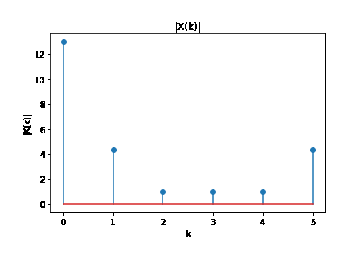
\includegraphics[width=7cm]{./figures/abs_X(k).eps}
    \caption{Magnitude of X(k)}
    \label{|X(k)|}
\end{figure} \\
\newpage
\begin{figure}[h!]
    \centering
    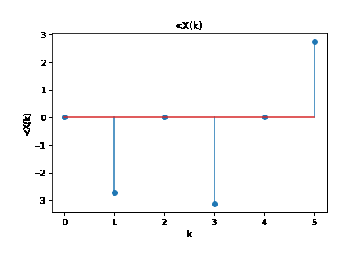
\includegraphics[width=9cm]{./figures/angle_X(k).eps}
    \caption{Phase of X(k)}
    \label{/_X(k)}
\end{figure}
\begin{figure}[h!]
    \centering
    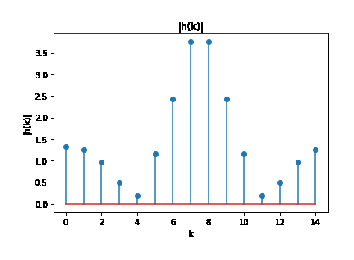
\includegraphics[width=9cm]{./figures/abs_h(k).eps}
    \caption{Magnitude of h(k)}
    \label{|h(k)|}
\end{figure} 
\begin{figure}[h!]
    \centering
    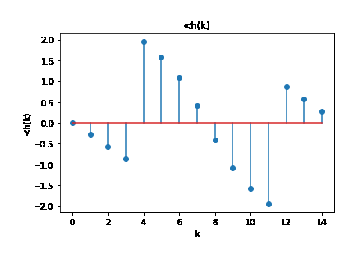
\includegraphics[width=9cm]{./figures/angle_h(k).eps}
    \caption{Phase of h(k)}
    \label{/_X(k)}
\end{figure}   

\end{document}